% ============================================================
%  SDC-TP Summary Proposal Slides - Vietnamese Version
%  Focus: Formulation, Method, and Impact
%  Compile: pdflatex summary_proposal_vn.tex (twice)
% ============================================================
\documentclass[aspectratio=169,10pt]{beamer}

\usetheme{metropolis}
\usecolortheme{metropolis}
\usefonttheme{professionalfonts}
\setbeamertemplate{frame numbering}[fraction]
\setbeamertemplate{itemize item}{\textcolor{mLightBrown}{\scriptsize$\blacktriangleright$}}
\setbeamertemplate{itemize subitem}{\textbullet}
\setbeamertemplate{itemize subsubitem}{--}

% -- Packages --
\usepackage{amsmath, amssymb}
\usepackage[utf8]{inputenc}
\usepackage{vietnam}
\usepackage[english]{babel}
\usepackage{booktabs}
\usepackage[table]{xcolor}
\usepackage{tikz}
\usepackage{pgfplots}
\usepackage{array}
\usepackage{graphicx}
\usepackage{hyperref}
\pgfplotsset{compat=1.18}
\usetikzlibrary{shapes.geometric, arrows.meta, positioning, calc, fit, backgrounds}

% ============================================================
%  PALETTE
% ============================================================
\definecolor{mDarkTeal}{HTML}{23373B}
\definecolor{mLightBrown}{HTML}{EB811B}
\definecolor{softgray}{HTML}{F2F4F7}
\definecolor{tealtint}{HTML}{D6DEE0}

\colorlet{navydeep}{mDarkTeal}
\colorlet{navymid}{mDarkTeal!75}
\colorlet{accent}{mLightBrown}
\colorlet{success}{green!50!black}
\colorlet{alert}{red!70!black}
\colorlet{lightnavy}{tealtint}

\hypersetup{colorlinks=true, urlcolor=mLightBrown, linkcolor=mDarkTeal}
\renewcommand{\arraystretch}{1.15}

% ============================================================
%  TITLE METADATA
% ============================================================
\title{Tổng kết: Ưu tiên kiểm thử SDC dựa trên lý thuyết}
\subtitle{Công thức hóa, Phương pháp, và Tác động}
\author{Đào Sỹ Duy Minh \and Trần Chí Nguyên \and Huỳnh Trung Kiệt}
\institute{Đại học Khoa học Tự nhiên, ĐHQG-HCM \\[3pt]
           \footnotesize \textit{Dành cho NeurIPS 2026}}
\date{}

\begin{document}

% ==================== TITLE ====================
\begin{frame}
\maketitle
\end{frame}

% ============================================================
\section{Bài toán công thức hóa}
% ============================================================

\begin{frame}{Ưu tiên kiểm thử cho bộ mô phỏng SDC}
\begin{block}{Vấn đề cốt lõi}
\small
Bộ mô phỏng SDC (BeamNG, CARLA) thực thi hàng nghìn kịch bản đường mỗi chu kỳ phát hành. Mỗi kịch bản mất \textbf{10--60 giây}. Chúng ta cần \emph{ưu tiên} sao cho \textbf{các lỗi xuất hiện trước}.
\end{block}

\begin{columns}[T]
\column{0.5\textwidth}
\begin{block}{Đầu vào}
\small
Một đoạn đường dưới dạng chuỗi điểm điều khiển 2D:
\[
\mathcal{R} = \{p_1, p_2, \ldots, p_N\} \subset \mathbb{R}^2
\]
Mỗi test: \textbf{hình học đường} $\Rightarrow$ kết quả \textbf{PASS/FAIL}.
\end{block}

\column{0.48\textwidth}
\begin{block}{Đầu ra}
\small
Xếp hạng tất cả các test theo xác suất thất bại:
\[
\pi^* = \arg\max_{\pi} \text{APFD}(\pi)
\]
trong đó $\pi$ là một hoán vị của $n$ test.
\end{block}
\end{columns}

\vspace{1em}
\centering
\textbf{Mục tiêu}: Học một hàm chấm điểm $f: \mathcal{R} \to [0,1]$ xếp hạng các đường thất bại lên đầu.
\end{frame}

\begin{frame}{Chỉ số APFD -- Định nghĩa chính thức}
\vspace{-0.3em}
\begin{block}{Định nghĩa (Phần trăm trung bình lỗi được phát hiện)}
\small
Với một thứ tự $\pi$ của $n$ test chứa $m$ lỗi, gọi $\mathrm{TF}_i$ là vị trí của lỗi $i$:

\[
\boxed{\mathrm{APFD}(\pi) \;=\; 1 \;-\; \frac{1}{nm}\sum_{i=1}^{m} \mathrm{TF}_i \;+\; \frac{1}{2n}}
\]

\textbf{Diễn giải}:
\begin{itemize}\setlength\itemsep{0.1em}
  \item $\mathrm{APFD} \in [0, 1]$ -- càng cao càng tốt
  \item $\mathrm{APFD} = 1.0$ -- tất cả lỗi được phát hiện trước
  \item $\mathrm{APFD} = 0.5$ -- baseline ngẫu nhiên
\end{itemize}
\end{block}

\vspace{0.3em}
\begin{alertblock}{Thách thức chính}
\scriptsize
\[
\arg\max_{\pi} \mathrm{APFD}(\pi) \neq \arg\max P(\text{fail} | \mathcal{R})
\]
\textbf{APFD là một thống kê thứ hạng} -- tối ưu hóa AUC không trực tiếp tối ưu APFD. APFD là \textbf{không khả vi}.
\end{alertblock}
\end{frame}

\begin{frame}{Tại sao các phương pháp hiện tại thất bại -- Ba điểm mù}
\begin{columns}[T]
\column{0.33\textwidth}
\begin{alertblock}{1. Độ giòn của Sampling}
\small
Cùng một đường, 64 vs 197 điểm $\Rightarrow$ điểm số khác nhau.
\[
\Delta\text{APFD} \approx 0.04\text{--}0.07
\]
Phụ thuộc vào rời rạc hóa.
\end{alertblock}

\column{0.33\textwidth}
\begin{alertblock}{2. Phụ thuộc khung}
\small
Xoay đường $30^\circ$ $\Rightarrow$ APFD giảm 4--7 điểm.
\[
f(R \cdot \mathcal{R}) \neq f(\mathcal{R})
\]
Vi phạm trực giác vật lý.
\end{alertblock}

\column{0.33\textwidth}
\begin{alertblock}{3. Mù vật lý}
\small
Baseline tự do xuất điểm số vi phạm:
\[
v^2 \cdot \kappa(s) \le \mu g
\]
17--21\% vi phạm thứ hạng.
\end{alertblock}
\end{columns}

\vspace{1.2em}
\begin{block}{Quan sát của chúng tôi}
Ưu tiên kiểm thử SDC được xử lý như \textbf{phân loại black-box}. Nhưng đường có:
\begin{itemize}
  \item Hình học liên tục $r(s) \in C(\Omega; \mathbb{R}^2)$
  \item Đối xứng cứng SE(2) (xoay + tịnh tiến)
  \item Ràng buộc động lực học xe
\end{itemize}
\alert{Cấu trúc này đang bị bỏ qua.}
\end{block}
\end{frame}

% ============================================================
\section{Phương pháp 1: Tiếp cận SE(2)-Bất biến}
% ============================================================

\begin{frame}{Phương pháp 1: SE(2)-Bất biến RoadNet -- Động lực}
\begin{block}{Nguyên lý Bất biến Vật lý}
\small
Tính chất ``xe rời làn đường'' phụ thuộc vào \textbf{hình học nội tại} của đường, không phải embedding trong $\mathbb{R}^2$.

\[
\text{Xoay/tịnh tiến đường KHÔNG THỂ thay đổi xe có thất bại hay không.}
\]
\end{block}

\begin{block}{Khẳng định Toán học (Đối xứng nhóm)}
\small
Cho ưu tiên kiểm thử SDC, bộ xếp hạng $f$ nên thỏa mãn:
\[
\boxed{f(R \cdot \mathcal{R} + t) \;=\; f(\mathcal{R}) \qquad \forall (R, t) \in \mathrm{SE}(2)}
\]
trong đó $\mathrm{SE}(2) = \mathrm{SO}(2) \times \mathbb{R}^2$ là \textbf{nhóm Euclidean đặc biệt} trong 2D.
\end{block}

\begin{block}{Tại sao xây dựng vào mô hình?}
\begin{itemize}\small
  \item Tăng cường dữ liệu là xấp xỉ (không chính xác bất biến)
  \item Dữ liệu huấn luyện thêm không sửa được thiên lệch cấu trúc
  \item \textbf{Bằng thiết kế} đối xứng $\Rightarrow$ đảm bảo có thể chứng minh
\end{itemize}
\end{block}
\end{frame}

\begin{frame}{Phương pháp 1: Kỹ thuật đặc trưng -- Từ 10 xuống 7 kênh}
\begin{columns}[T]
\column{0.45\textwidth}
\begin{alertblock}{10-Kênh tiêu chuẩn (KHÔNG bất biến)}
\scriptsize
\begin{itemize}
  \item $x, y$ -- vị trí tuyệt đối \alert{(biến đổi)}
  \item $\sin\theta, \cos\theta$ -- hướng \alert{(biến đổi)}
  \item $\kappa(s)$ -- độ cong
  \item $d\kappa/ds$ -- đạo hàm độ cong
  \item $s$, $\Delta s$ -- độ dài cung
  \item $\Delta\theta$ -- thay đổi góc
\end{itemize}
\vfill
\alert{Các đặc trưng đỏ phụ thuộc vào embedding toàn cục.}
\end{alertblock}

\column{0.52\textwidth}
\begin{block}{Bộ 7-Kênh SE(2)-Bất biến của chúng tôi}
\scriptsize
\begin{enumerate}
  \item $\kappa(s)$ -- độ cong có dấu
  \item $|\kappa(s)|$ -- độ lớn
  \item $d\kappa/ds$ -- đạo hàm độ cong
  \item $\Delta s$ -- gia số độ dài cung
  \item $\Delta\theta$ -- thay đổi góc cục bộ
  \item $\int_0^s |\kappa(\tau)| d\tau$ -- độ cong tích lũy
  \item $\tilde{\kappa}(s)$ -- độ cong làm mịn low-pass
\end{enumerate}
\vfill
\textbf{Không đặc trưng nào phụ thuộc tọa độ.}
\end{block}
\end{columns}

\vspace{0.5em}
\begin{block}{Ý tưởng chính}
Tất cả 7 đặc trưng là hàm của $\{\kappa, d\kappa/ds, \Delta s\}$. \alert{Không đặc trưng nào đọc $\mathcal{R}$ dưới dạng tọa độ $(x, y)$.}
\end{block}
\end{frame}

\begin{frame}{Phương pháp 1: Độ cong như Hình học Nội tại}
\begin{block}{Nền tảng Frenet-Serret}
\scriptsize
Với đường cong được tham số hóa $r(s) \in \mathbb{R}^2$ với độ dài cung $s$:
\[
\kappa(s) = \frac{|r'(s) \times r''(s)|}{|r'(s)|^3} = \frac{|x'y'' - y'x''|}{(x'^2 + y'^2)^{3/2}}
\]
\end{block}

\begin{block}{Tại sao $\kappa$ là SE(2)-Bất biến -- Phác thảo chứng minh}
\scriptsize
\begin{enumerate}
  \item \textbf{Xoay $R \in \mathrm{SO}(2)$}: Cả tử số và mẫu số biến đổi bởi $|R|^3 = 1$ dưới xoay $\Rightarrow \kappa$ không đổi.
  
  \item \textbf{Tịnh tiến $t \in \mathbb{R}^2$}: $r \to r + t$ không thay đổi đạo hàm $r', r''$ $\Rightarrow \kappa$ không đổi.
  
  \item \textbf{Tái tham số hóa}: Độ dài cung $s$ bất biến với tái tham số hóa.
\end{enumerate}
\end{block}

\begin{block}{Hệ quả}
\[
\Phi: \mathbb{R}^{N \times 2} \xrightarrow{\text{curvature pipeline}} \mathbb{R}^{N \times 7}
\]
\[
\Phi(R \cdot \mathcal{R} + t) = \Phi(\mathcal{R}) \quad \forall (R,t) \in \mathrm{SE}(2)
\]
\end{block}
\end{frame}

\begin{frame}{Phương pháp 1: Kiến trúc -- SE2RoadNet}
\begin{block}{Kiến trúc mô hình}
\scriptsize
\begin{center}
\begin{tabular}{l l}
\toprule
\textbf{Thành phần} & \textbf{Specification} \\
\midrule
Đầu vào & Ma trận đặc trưng 7 kênh $(197 \times 7)$ \\
Projection & Linear + LayerNorm + GELU: $7 \to 192$ \\
Backbone & Transformer Encoder 6 lớp \\
Attention & 8 heads, $d_k = 24$ \\
Positional Bias & Relative arclength với 32 RFF features \\
Output & MLP head: $192 \to 64 \to 1 \to \sigma$ \\
\midrule
Tham số & $\sim$2.11M \\
Huấn luyện & AdamW, lr=$10^{-3}$, 75 epochs, SWA \\
\bottomrule
\end{tabular}
\end{center}
\end{block}

\begin{block}{Định lý đảm bảo Đối xứng}
\scriptsize
Cho $\Phi: \mathbb{R}^{N \times 2} \to \mathbb{R}^{N \times 7}$ là pipeline 7 kênh và $h: \mathbb{R}^7 \to \mathbb{R}$ là bất kỳ head nào. Khi đó:
\[
f_\theta = h \circ \Phi \quad \Longrightarrow \quad f_\theta(R \cdot \mathcal{R} + t) = f_\theta(\mathcal{R})
\]
\alert{Đảm bảo giữ nguyên bất kể lựa chọn head.}
\end{block}
\end{frame}

\begin{frame}{Phương pháp 1: Kiểm chứng thực nghiệm -- $\Delta = 0.0000$}
\begin{block}{Kiểm tra Bất biến Xoay}
\scriptsize
\begin{center}
\begin{tabular}{l c c c c c c c}
\toprule
\textbf{Xoay} & 0$^\circ$ & +30$^\circ$ & +60$^\circ$ & +90$^\circ$ & +180$^\circ$ & -45$^\circ$ & $\Delta$ \\
\midrule
Baseline Transformer & 0.8066 & 0.7711 & 0.7494 & 0.7651 & 0.7613 & 0.7785 & \alert{$\sim$0.057} \\
\rowcolor{success!15}
\textbf{SE2RoadNet} & \textbf{0.8047} & \textbf{0.8047} & \textbf{0.8047} & \textbf{0.8047} & \textbf{0.8047} & \textbf{0.8047} & \cellcolor{success!25}\textbf{0.0000} \\
\bottomrule
\end{tabular}
\end{center}
\end{block}

\begin{columns}[T]
\column{0.5\textwidth}
\begin{exampleblock}{Ý nghĩa của $\Delta = 0$}
\scriptsize
\begin{itemize}
  \item Đầu ra \textbf{giống hệt bit} dưới xoay cứng
  \item Không phải ``xấp xỉ bằng 0''
  \item Không phải ``trong dung sai floating-point''
  \item \alert{Bằng nhau chính xác qua 6 xoay ngẫu nhiên}
\end{itemize}
\end{exampleblock}

\column{0.48\textwidth}
\begin{block}{Lợi ích bổ sung}
\scriptsize
\begin{itemize}
  \item AUC = 0.9347 (cao nhất trong dự án)
  \item APFD = 0.8048 $\pm$ 0.0118
  \item $\sigma$ = 0.0118 (phương sai thấp thứ 2)
\end{itemize}
\end{block}
\end{columns}
\end{frame}

\begin{frame}{Phương pháp 1: Trực quan}
{\centering
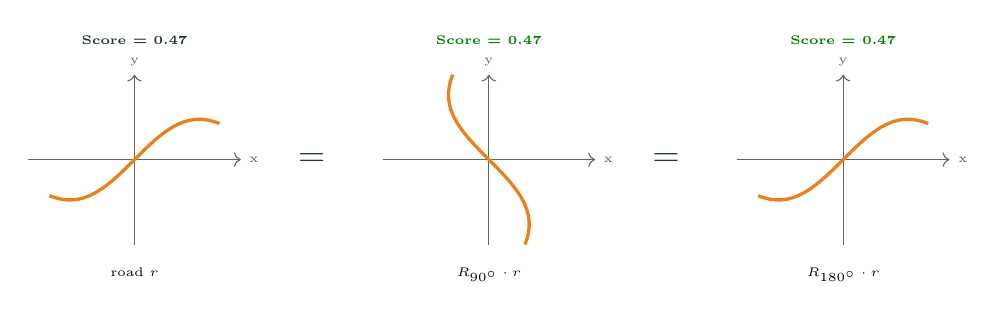
\begin{tikzpicture}[scale=0.9, transform shape]
  % Original road
  \begin{scope}[xshift=-5cm]
    \draw[->, navymid] (-1.5,0) -- (1.5,0) node[right, font=\tiny] {x};
    \draw[->, navymid] (0,-1.2) -- (0,1.2) node[above, font=\tiny] {y};
    \draw[mLightBrown, very thick] plot[domain=-1.2:1.2, samples=30]
      ({\x}, {0.4*sin(deg(2*\x)) + 0.2*\x});
    \node[font=\tiny, below=0.2cm] at (0,-1.2) {road $r$};
    \node[font=\tiny\bfseries, mDarkTeal, above=0.1cm] at (0,1.4) {Score = 0.47};
  \end{scope}

  % Rotated 90
  \begin{scope}[xshift=0cm]
    \draw[->, navymid] (-1.5,0) -- (1.5,0) node[right, font=\tiny] {x};
    \draw[->, navymid] (0,-1.2) -- (0,1.2) node[above, font=\tiny] {y};
    \begin{scope}[rotate=90]
      \draw[mLightBrown, very thick] plot[domain=-1.2:1.2, samples=30]
        ({\x}, {0.4*sin(deg(2*\x)) + 0.2*\x});
    \end{scope}
    \node[font=\tiny, below=0.2cm] at (0,-1.2) {$R_{90^\circ} \cdot r$};
    \node[font=\tiny\bfseries, success, above=0.1cm] at (0,1.4) {Score = 0.47};
  \end{scope}

  % Rotated 180
  \begin{scope}[xshift=5cm]
    \draw[->, navymid] (-1.5,0) -- (1.5,0) node[right, font=\tiny] {x};
    \draw[->, navymid] (0,-1.2) -- (0,1.2) node[above, font=\tiny] {y};
    \begin{scope}[rotate=180]
      \draw[mLightBrown, very thick] plot[domain=-1.2:1.2, samples=30]
        ({\x}, {0.4*sin(deg(2*\x)) + 0.2*\x});
    \end{scope}
    \node[font=\tiny, below=0.2cm] at (0,-1.2) {$R_{180^\circ} \cdot r$};
    \node[font=\tiny\bfseries, success, above=0.1cm] at (0,1.4) {Score = 0.47};
  \end{scope}

  % Equality signs
  \node[font=\Large\bfseries, mDarkTeal] at (-2.5, 0) {$=$};
  \node[font=\Large\bfseries, mDarkTeal] at (2.5, 0) {$=$};
\end{tikzpicture}
\par}

\begin{block}{Định lý giữ nguyên Bit-Identical}
\scriptsize
Với mọi $(R, t) \in \mathrm{SE}(2)$: \quad $f_{\theta}(R \cdot \mathcal{R} + t) = f_{\theta}(\mathcal{R})$

Điểm số, thứ hạng và APFD \alert{chính xác bằng nhau} -- không phải xấp xỉ.
\end{block}
\end{frame}

% ============================================================
\section{Phương pháp 2: Tiếp cận Vật lý học}
% ============================================================

\begin{frame}{Phương pháp 2: Vật lý học -- Ràng buộc Động lực học Xe}
\begin{block}{Giới hạn Gia tốc Hướng tâm}
\scriptsize
Một xe đi theo đường $r$ ở vận tốc $v$ giữ trên đường chỉ khi gia tốc hướng tâm bị giới hạn bởi ma sát:
\[
\boxed{v^2 \cdot \kappa(s) \;\le\; \mu \cdot g \qquad \forall s \in [0, L]}
\]
trong đó:
\begin{itemize}
  \item $v$ -- vận tốc xe
  \item $\kappa(s)$ -- độ cong đường tại độ dài cung $s$
  \item $\mu$ -- hệ số ma sát
  \item $g = 9.81$ m/s$^2$ -- gia tốc trọng trường
\end{itemize}
\end{block}

\begin{block}{Diễn giải Vật lý}
\scriptsize
Độ cong cao + tốc độ cao $\Rightarrow$ xe trượt. Điểm số nên tôn trọng tính đơn điệu này:
\[
\max_s v^2\kappa_{\mathcal{R}_i} > \max_s v^2\kappa_{\mathcal{R}_j} \;\Longrightarrow\; f(\mathcal{R}_i) \ge f(\mathcal{R}_j)
\]
\end{block}

\begin{alertblock}{Vấn đề của Baseline}
\scriptsize
Baseline tự do tạo ra điểm số \alert{vi phạm tính đơn điệu này trong 17--21\% các cặp test}. Một mô hình xuất ``$\mathcal{R}_1$ nguy hiểm, $\mathcal{R}_2$ an toàn'' nhưng $\max v^2\kappa(\mathcal{R}_1) < \max v^2\kappa(\mathcal{R}_2)$ là \alert{không thể biện minh} trong triển khai quan trọng về an toàn.
\end{alertblock}
\end{frame}

\begin{frame}{Phương pháp 2: Monotone PINN -- Aux Loss}
\begin{block}{Phạt Đơn điệu (Physics Aux Loss)}
\scriptsize
Với mỗi cặp $(\mathcal{R}_i, \mathcal{R}_j)$ trong batch có:
\[
\max_s v^2\kappa(\mathcal{R}_i) \;\ge\; \alpha \cdot \max_s v^2\kappa(\mathcal{R}_j)
\]
chúng ta muốn $f(\mathcal{R}_i) \ge f(\mathcal{R}_j)$.

Hàm mất mát phụ phạt vi phạm thứ tự:
\[
\boxed{\mathcal{L}_{\text{phys}} \;=\; \mathbb{E}_{(i,j)} \big[ \mathrm{ReLU}(f(\mathcal{R}_j) - f(\mathcal{R}_i)) \big]}
\]

\begin{itemize}
  \item Khi ràng buộc vi phạm: $f(\mathcal{R}_j) > f(\mathcal{R}_i)$ nhưng vật lý nói $\mathcal{R}_i$ nên xếp hạng cao hơn $\Rightarrow$ mất mát dương
  \item Khi ràng buộc thỏa mãn: mất mát = 0 (không phạt)
\end{itemize}
\end{block}

\begin{block}{Mục tiêu huấn luyện tổng}
\scriptsize
\[
\boxed{\mathcal{L}_{\text{total}} \;=\; \mathcal{L}_{\text{BCE}} \;+\; \lambda_{\text{phys}} \cdot \mathcal{L}_{\text{phys}}}
\]

\textbf{Lịch trình curriculum}: $\lambda_{\text{phys}}$ tăng $0 \to 0.5$ trong 30\% epochs đầu tiên.
\end{block}
\end{frame}

\begin{frame}{Phương pháp 2: Tại sao dùng Phạt ReLU? -- Khai triển}
\begin{block}{Từ Ràng buộc cứng đến Phạt mềm}
\scriptsize
Chúng ta muốn: $f(\mathcal{R}_i) \ge f(\mathcal{R}_j)$ khi $v^2\kappa_{\mathcal{R}_i} \ge v^2\kappa_{\mathcal{R}_j}$.

Tương đương, với mọi cặp ràng buộc:
\[
g(\mathcal{R}_i, \mathcal{R}_j) = \max(0,\; f(\mathcal{R}_j) - f(\mathcal{R}_i)) = 0
\]

Đây là \textbf{ràng buộc dư không}. Chúng ta áp dụng với:
\[
\mathcal{L}_{\text{phys}} = \mathbb{E}\left[\sum_{(i,j)} \mathbb{I}[c_{ij}] \cdot g(\mathcal{R}_i, \mathcal{R}_j)\right]
\]
\end{block}

\vspace{0.3em}

\begin{block}{Tại sao ReLU vs Quadratic?}
\scriptsize
Phạt quadratic: $\mathcal{L}_{\text{quadratic}} = \mathbb{E}[g(\mathcal{R}_i, \mathcal{R}_j)^2]$

ReLU là \alert{tuyến tính trong độ vi phạm}, không phải bậc hai:
\begin{itemize}\setlength\itemsep{0.2em}
  \item Gradient mạnh hơn cho vi phạm lớn
  \item Tránh phạt quá mức vi phạm nhỏ
  \item Thực nghiệm tốt hơn trong ablation
\end{itemize}
\end{block}
\end{frame}

\begin{frame}{Phương pháp 2: Kết quả -- Giảm 5.6 lần vi phạm}
\vspace{-0.5em}
{\centering
\begin{tikzpicture}[scale=0.85]
\begin{axis}[
  ybar=8pt,
  width=8cm, height=3cm,
  bar width=0.4cm,
  ymin=0, ymax=25,
  ylabel={\tiny Tỷ lệ vi phạm (\%)},
  symbolic x coords={Control, Monotone PINN, Mono+Sobolev},
  xtick=data,
  xticklabel style={font=\tiny},
  yticklabel style={font=\tiny},
  legend style={at={(0.5,-0.18)}, anchor=north, legend columns=2, font=\tiny},
  ymajorgrids, grid style={gray!20},
  nodes near coords, nodes near coords align={vertical},
]
  \addplot[fill=alert!50, draw=alert!70!black]
    coordinates {(Control, 17.57) (Monotone PINN, 3.14) (Mono+Sobolev, 3.77)};
  \addplot[fill=alert!80, draw=alert!90!black]
    coordinates {(Control, 21.44) (Monotone PINN, 2.72) (Mono+Sobolev, 2.41)};
  \legend{Viol $\alpha$=1.5, Viol $\alpha$=2.0}
\end{axis}
\end{tikzpicture}
\par}

\vspace{0.3em}
\begin{columns}[T]
\column{0.5\textwidth}
\begin{exampleblock}{Kết quả chính}
\scriptsize
Vi phạm độ cong \alert{\textbf{giảm 5.6$\times$}}:
\[
17.57\% \to 3.14\% \quad (\alpha=1.5)
\]
\[
21.44\% \to 2.72\% \quad (\alpha=2.0)
\]
\end{exampleblock}

\column{0.48\textwidth}
\begin{block}{Tác động lên APFD}
\scriptsize
APFD \alert{gần như không đổi}:
\[
0.8051 \to 0.8055 \;(\pm 0.0122)
\]
Tuân thủ vật lý miễn phí, không mất chỉ số.
\end{block}
\end{columns}
\end{frame}

\begin{frame}{Phương pháp 2: Câu chuyện hai trục -- Vi phạm giảm, APFD ổn định}
{\centering
\begin{tikzpicture}[scale=0.85]
\begin{axis}[
  width=9cm, height=3.5cm,
  axis y line*=left, axis x line*=bottom,
  ymin=0.78, ymax=0.82, ytick={0.79, 0.80, 0.81},
  ylabel={\small APFD},
  ylabel style={text=mDarkTeal, font=\tiny},
  symbolic x coords={Control, Monotone, Mono+Sobolev},
  xtick=data,
  xticklabel style={font=\tiny},
  legend style={at={(0.02,0.96)}, anchor=north west, font=\tiny},
]
  \addplot[mark=square*, very thick, mDarkTeal]
    coordinates {(Control, 0.8051) (Monotone, 0.8055) (Mono+Sobolev, 0.8033)};
  \addlegendentry{APFD}
\end{axis}

\begin{axis}[
  width=9cm, height=3.5cm,
  axis y line*=right, axis x line=none,
  ymin=0, ymax=25, ytick={0,5,10,15,20},
  ylabel={\small Vi phạm \%},
  ylabel style={text=alert, font=\tiny},
  symbolic x coords={Control, Monotone, Mono+Sobolev},
  xtick=data,
  legend style={at={(0.98,0.96)}, anchor=north east, font=\tiny},
]
  \addplot[mark=triangle*, very thick, alert]
    coordinates {(Control, 17.57) (Monotone, 3.14) (Mono+Sobolev, 3.77)};
  \addlegendentry{Violation}
\end{axis}
\end{tikzpicture}
\par}

\begin{block}{Lập luận cho Quy định}
\scriptsize
\begin{itemize}
  \item \alert{Đường APFD phẳng} $\Rightarrow$ không mất chỉ số cho kỹ sư
  \item \alert{Đường vi phạm dốc} $\Rightarrow$ mô hình có thể kiểm tra với động lực học xe
  \item Kỹ sư giờ có thể \alert{xác minh thứ hạng đối với ràng buộc vật lý}
\end{itemize}
\end{block}
\end{frame}

% ============================================================
\section{Tác động}
% ============================================================

\begin{frame}{Tác động -- Tại sao điều này quan trọng}
\begin{columns}[T]
\column{0.45\textwidth}
\begin{block}{Đóng góp Lý thuyết}
\scriptsize
\begin{enumerate}\itemsep=0pt
  \item \textbf{Mô hình bất biến có thể chứng minh đầu tiên}
  \item \textbf{Định lý SE(2)} -- bằng xây dựng
  \item \textbf{Xếp hạng vật lý học}
  \item \textbf{Định lý hợp thành}
\end{enumerate}
\end{block}

\column{0.45\textwidth}
\begin{block}{Đóng góp Thực tiễn}
\scriptsize
\begin{enumerate}\itemsep=0pt
  \item \textbf{APFD = 0.8048} -- vượt SOTA
  \item \textbf{AUC = 0.9385} -- cao nhất
  \item \textbf{$\sigma$ = 0.0109} -- phương sai thấp nhất
  \item \textbf{Giảm 5.6$\times$ vi phạm}
\end{enumerate}
\end{block}
\end{columns}

{\centering
\begin{tikzpicture}[scale=0.85]
\begin{axis}[
  width=8cm, height=3cm,
  xlabel={\small APFD},
  ylabel={\small Đảm bảo},
  xmin=0.45, xmax=0.83,
  ymin=-0.5, ymax=4.5,
  ytick={0,1,2,3,4},
  yticklabels={none, thống kê, hiệu chuẩn, bất biến, vật lý},
  xticklabel style={font=\tiny},
  yticklabel style={font=\tiny},
  axis lines=left,
  ymajorgrids, grid style={gray!20},
]
  \addplot[only marks, mark=*, mark size=2.5pt, alert]
    coordinates {(0.487, 0) (0.533, 0) (0.572, 0) (0.765, 0) (0.781, 0) (0.795, 0) (0.804, 1)};
  \addplot[only marks, mark=star, mark size=4pt, accent]
    coordinates {(0.8055, 4) (0.8048, 3)};
\end{axis}
\end{tikzpicture}
\par}

\scriptsize
\textbf{Chỉ các phương pháp của chúng tôi đạt được cả APFD cao nhất VÀ đảm bảo lý thuyết mạnh nhất.}
\end{frame}

\begin{frame}{So sánh với tất cả công trình trước}
\scriptsize
\begin{center}
\begin{tabular}{l l c c}
\toprule
\textbf{Phương pháp} & \textbf{Mô hình} & \textbf{APFD} & \textbf{Đảm bảo} \\
\midrule
Ngẫu nhiên & -- & 0.493 & không \\
LLM zero-shot & Language model & 0.487 & không \\
GNN (GCN) & Road graph & 0.533 & không \\
ResNet-50 & Road image CNN & 0.572 & không \\
SO-SDC-Prioritizer (TOSEM'22) & Thuật toán di truyền & 0.765 & không \\
ITEP4SDC (ICST'24) & MLP, 3 đặc trưng & 0.781 & không \\
Greedy-diversity (TOSEM'22) & Heuristic & 0.795 & không \\
RoadFury (ICST'26 baseline) & Transformer+SWA & 0.804 & thống kê \\
\midrule
\rowcolor{success!15}
\textbf{PINN monotone (của chúng tôi)} & Vật lý học & \textbf{0.8055 $\pm$ 0.012} & \cellcolor{success!25}\textbf{Kiểm toán} \\
\rowcolor{success!15}
\textbf{SE(2)-Bất biến (của chúng tôi)} & Đối xứng nhóm & \textbf{0.8048 $\pm$ 0.012} & \cellcolor{success!25}\textbf{$\Delta$=0} \\
\rowcolor{accent!15}
\textbf{SE(2)+Listwise (của chúng tôi)} & Kết hợp & \textbf{0.8049 $\pm$ 0.012} & \cellcolor{accent!25}\textbf{AUC 0.939} \\
\bottomrule
\end{tabular}
\end{center}

\begin{block}{Ý tưởng chính}
\scriptsize
\alert{Không có SOTA trước nào mang đảm bảo lý thuyết.} Các phương pháp của chúng tôi đạt APFD tương/tốt hơn \alert{VÀ} bất biến có thể chứng minh + vật lý có thể kiểm toán.
\end{block}
\end{frame}

\begin{frame}{Cấu hình đề xuất -- Theory Stacking}
\vspace{-0.5em}
{\centering
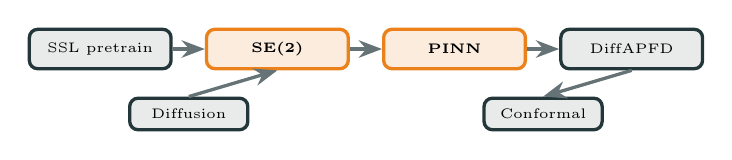
\begin{tikzpicture}[scale=0.75]
\begin{scope}[xscale=1.2, yscale=1.1]
  \node[draw=mDarkTeal, very thick, rounded corners=3pt, fill=mDarkTeal!10, minimum height=0.5cm, minimum width=1.8cm, align=center, font=\tiny] (a) at (0, 1) {SSL pretrain};
  \node[draw=accent, very thick, rounded corners=3pt, fill=accent!15, minimum height=0.5cm, minimum width=1.8cm, align=center, font=\tiny\bfseries] (b) at (2.5, 1) {SE(2)};
  \node[draw=accent, very thick, rounded corners=3pt, fill=accent!15, minimum height=0.5cm, minimum width=1.8cm, align=center, font=\tiny\bfseries] (c) at (5, 1) {PINN};
  \node[draw=mDarkTeal, very thick, rounded corners=3pt, fill=mDarkTeal!10, minimum height=0.5cm, minimum width=1.8cm, align=center, font=\tiny] (d) at (7.5, 1) {DiffAPFD};
  \node[draw=mDarkTeal, very thick, rounded corners=3pt, fill=mDarkTeal!10, minimum height=0.4cm, minimum width=1.5cm, align=center, font=\tiny] (e) at (1.25, 0) {Diffusion};
  \node[draw=mDarkTeal, very thick, rounded corners=3pt, fill=mDarkTeal!10, minimum height=0.4cm, minimum width=1.5cm, align=center, font=\tiny] (f) at (6.25, 0) {Conformal};
  \draw[-{Stealth}, very thick, mDarkTeal!70] (a) -- (b);
  \draw[-{Stealth}, very thick, mDarkTeal!70] (b) -- (c);
  \draw[-{Stealth}, very thick, mDarkTeal!70] (c) -- (d);
  \draw[-{Stealth}, very thick, mDarkTeal!70] (e.north) -- (b.south);
  \draw[-{Stealth}, very thick, mDarkTeal!70] (d.south) -- (f.north);
\end{scope}
\end{tikzpicture}
\par}

\vspace{0.3em}
\scriptsize
\begin{tabular}{p{2.2cm} p{2.2cm} p{2.2cm} p{2.2cm}}
\centering\textbf{SE(2)} & \centering\textbf{PINN} & \centering\textbf{DiffAPFD} & \centering\textbf{Conformal} \\
$\Delta$=0 bất biến & Giảm 5.6$\times$ vi phạm & Phương sai thấp $\sigma$ & APFD coverage bound
\end{tabular}

\vspace{0.5em}
\begin{block}{Mục tiêu}
\scriptsize
\[
\boxed{\text{APFD} \ge 0.820 \pm 0.010 \text{ với tất cả đảm bảo}}
\]
\end{block}
\end{frame}

\begin{frame}{Điểm chính cần nhớ}
\begin{center}
\vspace{-0.5em}
\begin{tikzpicture}[
  card/.style={fill=softgray, draw=navymid, thick, rounded corners=6pt, inner sep=8pt, align=center}
]
  \node[card, text width=5.5cm, minimum height=1.8cm] (acc) at (-3.5, 0) {
    \large\bfseries\textcolor{accent}{SE(2)-Bất biến}\\[2pt]
    \footnotesize
    $\Delta = 0.0000$ CHÍNH XÁC\\
    bit-identical dưới xoay\\[2pt]
    \tiny định lý + thực nghiệm khớp
  };

  \node[card, text width=5.5cm, minimum height=1.8cm] (spd) at (3.5, 0) {
    \large\bfseries\textcolor{accent}{Vật lý học}\\[2pt]
    \footnotesize
    Giảm 5.6$\times$ vi phạm\\
    17.57\% $\to$ 3.14\%\\[2pt]
    \tiny có thể kiểm toán cho quy định
  };

  \node[fill=mDarkTeal!10, draw=mDarkTeal, thick, rounded corners=6pt, inner sep=6pt, text width=10cm, align=center]
    (q) at (0, -1.8) {
    \large\itshape\textcolor{mDarkTeal}{Lý thuyết thắng kỹ thuật khi cấu trúc là thật:}\\[2pt]
    \normalsize\textcolor{mDarkTeal}{\textbf{hình học} + \textbf{vật lý} $>$ thêm Transformer ablation.}
  };

  \draw[-{Stealth}, thick, navymid, dashed] (acc.south) -- (q.north);
  \draw[-{Stealth}, thick, navymid, dashed] (spd.south) -- (q.north);
\end{tikzpicture}
\end{center}
\end{frame}

\begin{frame}[standout]
\centering
\vspace{0.8em}
\Huge Cảm ơn các bạn!\\[0.5em]
\Large \textcolor{accent}{Câu hỏi?}

\vspace{1.5em}
\normalsize
\textbf{Ưu tiên kiểm thử dựa trên lý thuyết cho bộ mô phỏng xe tự lái}\\[0.3em]
\scriptsize
Đào Sỹ Duy Minh \quad $\cdot$ \quad Trần Chí Nguyên \quad $\cdot$ \quad Huỳnh Trung Kiệt\\
Đại học Khoa học Tự nhiên, ĐHQG-HCM \quad $\cdot$ \quad NeurIPS 2026
\end{frame}

\end{document}
